\chapter{Spectral Method} \label{chap:spectral-method}
\section{Spectral Theory in Finite-Dimensional Normed Spaces}
Let $X$ be a finite dimensional normed space and $\hat{T}: X \to X$ a linear operator. Since any linear operator can be represented by a matrix, the spectral theory of $\hat{T}$ is essentially matrix eigenvalue theory. \cite{kreyszig_introductory_1978} Let $A$ be a matrix representation of $\hat{T}$, then we have the definition.

\begin{definition}
	An eigenvalue of a square matrix $A$ is a complex number $\lambda$ such that
	\[ Ax = \lambda x \]
	has a solution $x\neq 0$.This $x$ is called an \textbf{eigenvector} of $A$ corresponding to that eigenvalue $\lambda$.The set $\sigma(A)$ of all eigenvalues of $A$ is called the \textbf{spectrum} of $A$. Its complement $\rho(A) = \mathbb{C}-\sigma(A)$ in the complex plane is called the \textbf{resolvent} set of $A$.
\end{definition}

By choosing different bases in $X$, we can have different matrix representation of $\hat{T}$. We need to make sure the eigenvalues of a linear operator is independent of the basis chosen. Fortunately, a theorem ensures that.

\begin{theorem}
	All matrices representing a given linear operator $\hat{T}: X \to X$ on a finite dimensional normed space $X$ relative to various bases for $X$ have the same eigenvalues.
\end{theorem}


Moreover, we don't need to worry about the existence of eigenvalues of a linear operator. The following theorem shows the existence of them.
\begin{theorem}
	A linear operator on a finite dimensional complex normed space $X\neq{O}$ has at least one eigenvalue.
\end{theorem}


\section{Spectral Theory in Normed Spaces of Any Dimension}
Let $X\neq {0}$ be a complex normed space (could be any dimension), and $\hat{T}: D(\hat{T}) \to X$ with domain $D(\hat{T}) \subset X$. Again, we could define eigenvalues, and other related concepts in terms of the equation
\[ \hat{T}x = \lambda x \]

\begin{definition}
	Let $\hat{T}\neq{0}$ be a complex normed space and $\hat{T}: D(\hat{T}) \to X$ a linear operator with domain $D(\hat{T})\subset X$. A \textbf{regular value} $\lambda$ of $\hat{T}$ is a complex number such that
	\begin{itemize}
		\item [(R1)] $(\hat{T}-\lambda I)^{-1}$ exists,
		\item [(R2)] $(\hat{T}-\lambda I)^{-1}$ is bounded,
		\item [(R3)] $(\hat{T}-\lambda I)^{-1}$ is defined on a set which is dense in $X$,
	\end{itemize}

	The \textbf{resolvent set} $\rho(\hat{T})$ of $\hat{T}$ is the set of all regular values $\lambda$ of $\hat{T}$. Its complement $\sigma(\hat{T}) = \mathbb{C} - \rho(\hat{T})$ in the complex plane $\mathbb{C}$ is called the \textbf{spectrum} of $\hat{T}$, and a $\lambda\in \sigma(\hat{T})$ is called a \textbf{spectral value} of $\hat{T}$. Furthermore, the spectrum $\sigma(\hat{T})$ is partitioned into three disjoint sets as follows.
	\begin{itemize}
		\item The \textbf{point spectrum} or \textbf{discrete spectrum} $\sigma_p(\hat{T})$ is the set such that $(\hat{T}-\lambda I)^{-1}$ does not exist. A $\lambda\in\sigma_p(\hat{T})$ is called an \textbf{eigenvalue} of $\hat{T}$.
		\item The \textbf{continuous spectrum} $\sigma_c(\hat{T})$ is the set such that $(\hat{T}-\lambda I)^{-1}$ exists and satisfies (R3) but not (R2), that is, $(\hat{T}-\lambda I)^{-1}$ is unbounded.
		\item The \textbf{residual spectrum} $\sigma_r(\hat{T})$ is the set such that $(\hat{T}-\lambda I)^{-1}$ exists (and may be bounded or not) but does not satisfy (R3), that is, the domain of $(\hat{T}-\lambda I)^{-1}$ is not dense in X.
	\end{itemize}
\end{definition}

In practice, the eigenvalue problem in infinite dimension is difficult.
Therefore, the usual approach to the eigenvalue problem $\hat{T}x=\lambda x$ is to first discretize the operator $\hat{T}$ to an approximated matrix operator $T$, then the eigenvalue problem becomes,
\[ Tx = \lambda x \]

There are different ways to discretize the operator. For example, we can use finite difference, finite element and spectral element methods.

One important thing we need to keep in mind is that, the discretized version of the eigenvalue problem can have eigenvalues that are not in $\sigma(\hat{T})$. Those eigenvalues are called spurious eigenvalues, and this phenomenon is called spectral pollution. It is due to the improper discretization of the operators. We will discuss spectral pollution in the next section.

\section{Different Discretizations}
Spectral method is one of the best tools to solve PDE and ODE problems. \cite{trefethen_spectral_2000} The central idea of spectral method is by discretizing the equation, we can transform that to a linear system or an eigenvalue problem.

Here we reformulate the polynomial eigenvalue problem, Eq.~(\ref{eq:polynomial-eigenvalue-problem}) as the following,
\begin{equation} \label{eq:eigenvalue-problem}
	\mqty[ 0 & 1\\ \hat{M} & \hat{N} ]\mqty[ \tilde{v}\\ \omega \tilde{v}] = \omega\mqty[ \tilde{v}\\ \omega \tilde{v}]
\end{equation}
where the operators $\hat{M}$ and $\hat{N}$ are defined as
\begin{align*}
	\hat{M} & = -\left[(1-v_0^2)\pdv[2]{}{z}
		-\left(3v_0 + \frac{1}{v_0}\right)\pdv{v_0}{z}\pdv{}{z}
		- \left(1-\frac{1}{v_0^2}\right)\left(\pdv{v_0}{z}\right)^2
	- \left(v_0+\frac{1}{v_0}\right)\pdv[2]{v_0}{z}\right]  \\
	\hat{N} & = -2i\left(v_0\pdv{}{z} +\pdv{v_0}{z} \right)
\end{align*}
This becomes an ordinary algebraic eigenvalue problem if we discretize the operators and the function $\tilde{v}$. The following subsections discuss different discretizations of the problem.

\subsection{Finite Difference}
Consider equally spaced nodes on domain $[-1,1]$, $\{x_1, x_2, \dots, x_N\}$ with $x_{j+1}-x_{j} = h$ for each $j$, and the set of corresponding function values, $\{ f_1, f_2, \dots, f_N \}$. We can approximate the derivatives using second-order central difference formulas
\[
	\pdv{f}{z} = \frac{f_{j+1} - f_{j-1}}{2h}
	\qquad
	\pdv[2]{f}{z} = \frac{f_{j+1} -2f_{j} +f_{j-1}}{h^2}
\]

We can discretize the differentiation operators to the following matrices
\[
	\pdv{z} \rightarrow D = \frac{1}{2h}\begin{bmatrix}
		0      & 1      & 0      & \dots  & 0      \\
		-1     & \ddots & \ddots & \ddots & \vdots \\
		0      & \ddots & \ddots & \ddots & 0      \\
		\vdots & \ddots & \ddots & \ddots & 1      \\
		0      & \dots  & 0      & -1     & 0
	\end{bmatrix}
	\qquad
	\pdv[2]{z} \rightarrow  D^2 = \frac{1}{h^2}\begin{bmatrix}
		-2     & 1      & 0      & \dots  & 0      \\
		1      & \ddots & \ddots & \ddots & \vdots \\
		0      & \ddots & \ddots & \ddots & 0      \\
		\vdots & \ddots & \ddots & \ddots & 1      \\
		0      & \dots  & 0      & 1      & -2
	\end{bmatrix}
\]

Using these differentiation matrices, Eq.~(\ref{eq:eigenvalue-problem}) becomes
\begin{equation}
	\mqty[ O & I\\ M & N ]\mqty[ \mathbf{\tilde{v}}\\ \omega\mathbf{\tilde{v}} ] = \omega\mqty[ \mathbf{\tilde{v}}\\ \omega\mathbf{\tilde{v}} ]
\end{equation}
where $O$ is a zero matrix, $I$ is an identity matrix, and
\begin{align*}
	M = & -\text{diag}(1-\mathbf{v}_0^2)D^2
	+\text{diag}\left(3\mathbf{v}_0 + \frac{1}{\mathbf{v}_0}\right) (D\mathbf{v}_0)D
	+\text{diag}\left(1-\frac{1}{\mathbf{v}_0^2}\right)\left(D\mathbf{v}_0\right)^2     \\
	    & +\text{diag}\left(\mathbf{v}_0+\frac{1}{\mathbf{v}_0}\right)(D^2\mathbf{v}_0) \\
	N = & -2i\left(\text{diag}(\mathbf{v}_0)D + D\mathbf{v}_0 \right)
\end{align*}
Here we abused the notation for the purpose of convenience, $\mathbf{v}_0^2$ means squaring every component of $\mathbf{v}_0$, and $1/\mathbf{v}_0$ denotes 1 divided by all components of $\mathbf{v}_0$.

\subsubsection{Boundary Condition}
We impose Dirichlet boundary condition on the problem, meaning that $\tilde{v}(-1)=\tilde{v}(1)=0$. Further more, the differentiation matrices do not do well on the edges, so during the computation, we remove the first and last row of the differentiation matrices and the vectors $\mathbf{\tilde{v}}$ and $\mathbf{v}_0$. After the computation, we set $\tilde{v}_1=\tilde{v}_N = 0$.

\subsection{Spectral Element}
Suppose the basis functions are $\{u_k(z)\}_{k=1}^\infty$, then the eigenfunction $\tilde{v}$ can be approximated by finite amount of them, $\tilde{v}(z) = \sum_{k=1}^N c_ku_k(z)$ where $c_k$ are coefficients to be determined.

Then by multiplying $u_{i}$ to any term and integrate through the domain, we can discretize the equation. Using the notation of inner product $(f,g)=\int_{-1}^{1} dz fg$, we see that

\[ \int_{-1}^{1} dz \; u_i\tilde{v} = \sum_{j}(u_i,u_j)c_j \]
\[ \int_{-1}^{1} dz \; u_i\pdv{\tilde{v}}{z} = \sum_{j}\left(u_i,\pdv{u_j}{z}\right)c_j \]
\[ \int_{-1}^{1} dz \; u_i\pdv[2]{\tilde{v}}{z} = \sum_{j}\left(u_i,\pdv[2]{u_j}{z}\right)c_j \]

Suppose the basis functions are $\{u_k(z)\}_{k=1}^\infty$, then the eigenfunction $\tilde{v}$ can be approximated by finite amount of them, $\tilde{v}(z) = \sum_{k=1}^N c_ku_k(z)$ where $c_k$ are coefficients to be determined.

\begin{equation} \label{eq:eigenvalue-problem-SE}
	\mqty[ O & I\\ M & N ]\mqty[ \mathbf{c}\\ \omega\mathbf{c} ] = \omega\mqty[ \mathbf{c}\\ \omega\mathbf{c} ]
\end{equation}
where $O$ is a zero matrix, $I$ is an identity matrix, and
\begin{align*}
	M_{jk} & = -\int_{-1}^{1}dz \; u_{j} \left[(1-v_0^2)\pdv[2]{}{z}
		-\left(3v_0 + \frac{1}{v_0}\right)\pdv{v_0}{z}\pdv{}{z}
		- \left(1-\frac{1}{v_0^2}\right)\left(\pdv{v_0}{z}\right)^2
	- \left(v_0+\frac{1}{v_0}\right)\pdv[2]{v_0}{z}\right] u_{k}                        \\
	N_{jk} & = -2i\int_{-1}^{1}dz \; u_{j}\left(v_0\pdv{}{z} +\pdv{v_0}{z} \right)u_{k}
\end{align*}

\subsubsection{Boundary Conditions and Basis Function}
To satisfy the Dirichlet boundary condition, $\tilde{v}(\pm 1)=0$, we can choose a set of basis functions that satisfy the boundary condition $u_k(\pm 1)=0,\forall k\in\mathbb{N}$. For example, the sine functions
\[ u_n(z) = \sin(\frac{n\pi}{2}(z+1)), n\in\mathbb{N} \]
is a set of basis functions that satisfy the Dirichlet boundary condition.



\subsection{Finite Element}
Finite-element method is a generalization of the spectral element method. We are allow to use a set of basis functions similar to spectral method in a cell. The region consists of many of these cells.

The formulation is the same as Eq.~(\ref{eq:eigenvalue-problem-SE}). The only difference is that in finite-element we need to solve Eq.~(\ref{eq:eigenvalue-problem-SE}) simultaneously for all cells.

\subsubsection{Boundary Conditions and B-Spline}
The B-Spline is a commonly used basis function for finite-element method. B-Spline can be defined recursively starting with piecewise constants [reference needed]

\begin{equation}
	B_{i,0}(\xi) = \begin{cases}
		1, & \text{if } \xi_i\leq \xi \leq \xi_{i+1} \\
		0, & \text{otherwise}
	\end{cases}
\end{equation}
For $j\in\mathbb{N}$, they are defined by
\begin{equation}
	B_{i,j}(\xi) = \frac{\xi-\xi_i}{\xi_{i+j}-\xi_i}B_{i,j-1}(\xi)
	+ \frac{\xi_{i+j+1}-\xi}{\xi_{i+j+1}-\xi_{i+1}}B_{i+1,p-1}(\xi)
\end{equation}
where $\mathbf{\xi}=[\xi_0,\cdots,\xi_m]$ is called the knot vector, where $m=n+j+1$ where $n+1$ is the number of B-Splines and $j$ is the degree of B-Spline polynomials. The knot vector defines the shapes of the B-Splines, see Fig.~\ref{fig:bspline}. The variable $\xi$ is within the range $[\xi_0, \xi_m]$.

Any function $u(x)$ on $[\xi_0,\xi_N]$ can be approximated by
\[ u(x) \simeq \sum_{j=0}^{n} c_jB_{i,j}(x) \]

The Dirichlet boundary condition can be set by letting the coefficients of the first and last B-Spline to 0, $c_{0}=c_{n} = 0$, where $N$ is the number of B-Splines.

\begin{figure} [H]
	\centering
	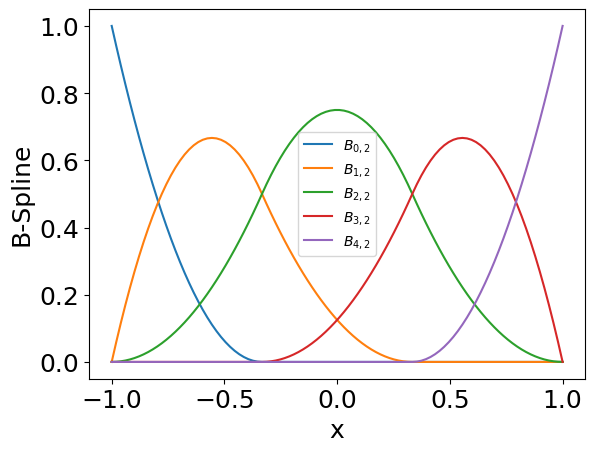
\includegraphics[width=0.7\linewidth]{figures/bspline}
	\caption{An example of open uniform quadratic B-Spline on $[-1,1]$. The knot vector is [-1,-1,-1,-1/3,1/3,1,1,1].}
	\label{fig:bspline}
\end{figure}



\section{Spectral Pollution and Spurious Modes}
In this section, we will discuss an important phenomenon we observe throughout the numerical experiments. It is the phenomenon of spectral pollution. Then we will provide a method to filter these spurious modes.

Spectral pollution refers to the phenomenon which some eigenvalues are not converging to the correct value when the mesh density is increased. When solving eigenvalue problems using spectral methods with finite difference or finite element approximations, spectral pollution might occur. \cite{llobet_spectral_1990}

\subsection{Finite Difference Discretization of Operators}
In this section, we are going to investigate the spectral pollution phenomenon when solving Eq.~(\ref{eq:constant-v-problem-dirichlet}) using spectral method.

The dispersion relation can be obtained by substituting $\tilde{v} = \exp(-i\omega t + kx)$ into Eq.~(\ref{eq:constant-v-problem-dirichlet}),
\begin{equation} \label{dispersion-relation}
	\omega = k(v_0 \pm 1)
\end{equation}

If we assume $v\sim \exp(ikx)$, and let $\beta\equiv kh/2$. Then in finite difference discretization scheme, the differential operators $\dv*[n]{z}$ are equivalent to the following factors \cite{llobet_spectral_1990},
\begin{align}
	 & G_0 = 1 \nonumber                                                              \\
	 & G_1 = [\exp(2i\beta)-\exp(-2i\beta)]/2h = (i/h)\sin(2\beta)
	\label{G-operator}                                                                \\
	 & G_2 = [\exp(2i\beta)-2-\exp(-2i\beta)]/h^2 = (2/h^2)(\cos(2\beta)-1) \nonumber
\end{align}


\subsection{Analysis of Numerical Spectrum}
\subsubsection{Discretize on the Same Grid}
Using the G-operator, Eq.~(\ref{G-operator}), the discretized equation of Eq.~(\ref{eq:constant-v-problem-dirichlet}) is
\begin{equation} \label{eq:discretized-eq-G}
	(\omega^2G_0 + \omega G_1 + G_2)\mathbf{\tilde{v}} = 0
\end{equation}
where $\mathbf{\tilde{v}}$ is the discretized vector of $\tilde{v}$.

Solving Eq.~(\ref{eq:discretized-eq-G}), we obtain the numerical dispersion relation,
\begin{equation} \label{dispersion-relation-G}
	\omega = \frac{2\sin(\beta)}{h}\left(v_0 \pm \sqrt{1 - v_0^2\sin[2](\beta)}\right)
\end{equation}

Given $h$ (fixed the mesh resolution), we see that
\begin{itemize}
	\item $\omega$ is real for all $k$ if $v_0 < 1$.
	\item $\omega$ is complex for large $k$, more specifically $k>h/2\arcsin(1/v_0)$, if $v_0 > 1$.
	\item For small $k$, meaning $k\to 0$, Eq.~(\ref{dispersion-relation-G}) is a good representation for the analytical dispersion relation, Eq.~(\ref{dispersion-relation}).
\end{itemize}
This explains why the spurious unstable modes occur when $v_0>1$.

\begin{figure}[H]
	\centering
	\begin{subfigure}[b]{0.5\linewidth}
		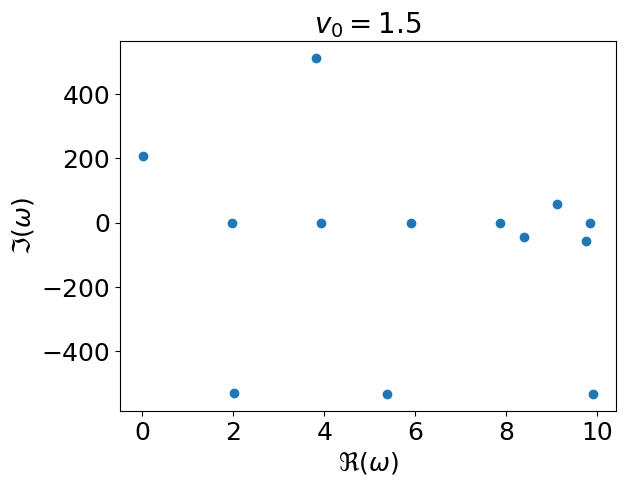
\includegraphics[width=\linewidth]{figures/eigvals-bad}
		\caption{Bad eigenvalues}
	\end{subfigure}%
	\begin{subfigure}[b]{0.5\linewidth}
		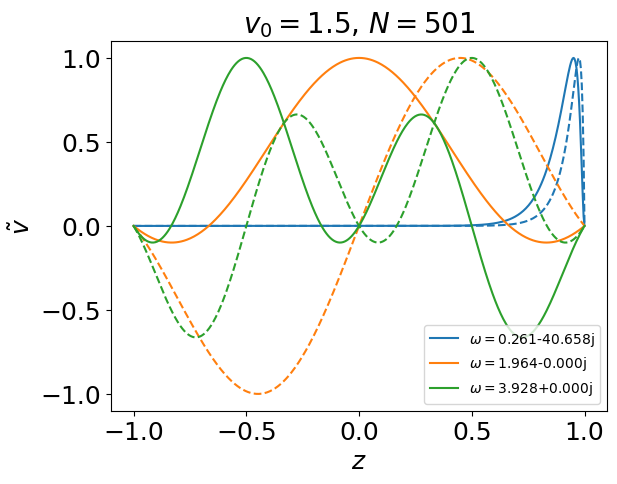
\includegraphics[width=\linewidth]{figures/eigvecs-bad}
		\caption{Bad eigenfunctions}
	\end{subfigure}
	\caption{Spurious modes.}
	\label{fig:results-bad}
\end{figure}

One way to filter the spurious modes is to remove all modes with $k>h/2 \arcsin(1/v_0)$, see Fig.~\ref{fig:results-filter-k}. However, this is not a good way to deal with general cases because it requires the solution to the discretized problem Eq.~(\ref{eq:discretized-eq-G}). For general problem with non-constant velocity profile, it is hard to solve the discretized problem directly.

\begin{figure}[H]
	\centering
	\begin{subfigure}[b]{0.5\linewidth}
		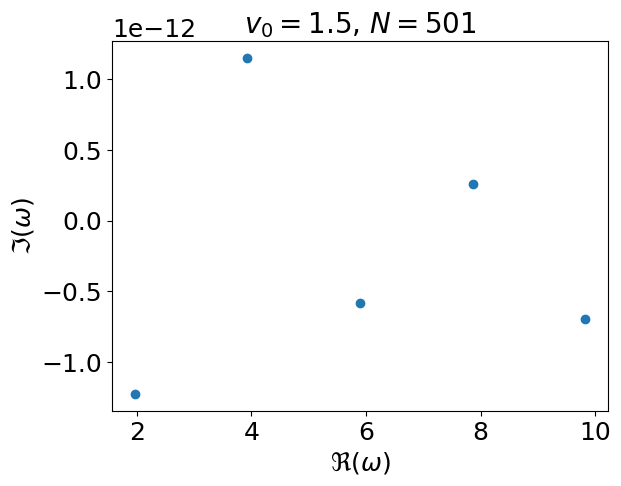
\includegraphics[width=\linewidth]{figures/eigvals-good}
		\caption{Good eigenvalues}
	\end{subfigure}%
	\begin{subfigure}[b]{0.5\linewidth}
		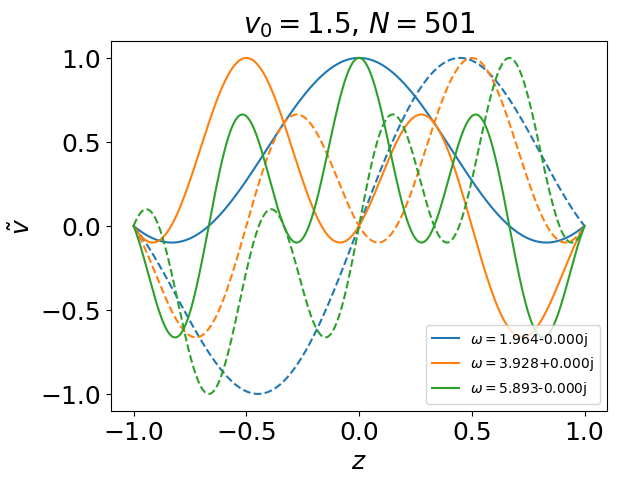
\includegraphics[width=\linewidth]{figures/eigvecs-good}
		\caption{Good eigenfunctions}
	\end{subfigure}
	\caption{Filter out the spurious modes with $k>h/2\arcsin(1/v_0)$.}
	\label{fig:results-filter-k}
\end{figure}

A better way to filter the spurious modes is by doing a "convergence test". Since the frequency Eq.~(\ref{dispersion-relation-G}) is changing with mesh resolution $h$. We can simply solve the discretized problem using spectral method under different mesh resolution. Then filter out the eigenmodes that are changing dramatically.
